\subsection{Comparison with theoretical models} \label{sec:WBoson_Results_ComparisonWithTheory}


The measurements of the \W boson production in \pPb collisions at \sqrtsnn=8.16~\TeV are compared to three NLO PDF calculations, one assuming no nuclear effects (CT14 PDF~\cite{CT14}) and two including nuclear modifications (CT14+EPPS16 nPDF~\cite{EPPS16} and CT14+nCTEQ15 nPDF~\cite{nCTEQ15}). The NLO PDF calculations are produced using the parton-level Monte Carlo program MCFM~\cite{MCFM}. The comparison between the PDF calculations and the data are shown in \fig{fig:CrossSection_WToMu_PA_Model} for the \W differential cross sections, in \fig{fig:ChargeAsymmetry_WToMu_PA_Model} for the muon charge asymmetry and in \fig{fig:ForwardBackwardRatio_WToMu_PA_Model} for the muon forward backward ratios. In all cases, the PDF calculations with (without) including nuclear modifications are displayed using dashed (continuos) lines and the corresponding PDF uncertainties are shown using hatched (filled) boxes.

As can be seen in \fig{fig:CrossSection_WToMu_PA_Model}, the \W cross section measurements at forward rapidity favor the PDF calculations including nuclear modifications, while at backward rapidity all three PDF calculations are in good agreement with the data. Moreover, in the case of the muon charge asymmetry shown in \fig{fig:ChargeAsymmetry_WToMu_PA_Model}, the results of the theory calculations derived using CT14 PDF only, and those including nuclear modifications described by EPPS16 nPDF, are in good agreement with the measurements while the CT14+nCTEQ15 nPDF calculations expect a slightly larger muon charge asymmetry in the most backward \etaCM bins. Finally, from the ratios of muon yields at forward over backward \etaCM displayed in \fig{fig:ForwardBackwardRatio_WToMu_PA_Model}, the nuclear PDF calculations describe much better the data compared to the free-nucleon PDF calculation. Considering the smaller size of the uncertainties compared to the theory uncertainties, the measurements have the potential to constrain the CT14+EPPS16 and the CT14+nCTEQ15 nPDF models.


\begin{figure}[htbp]
 \begin{center}
  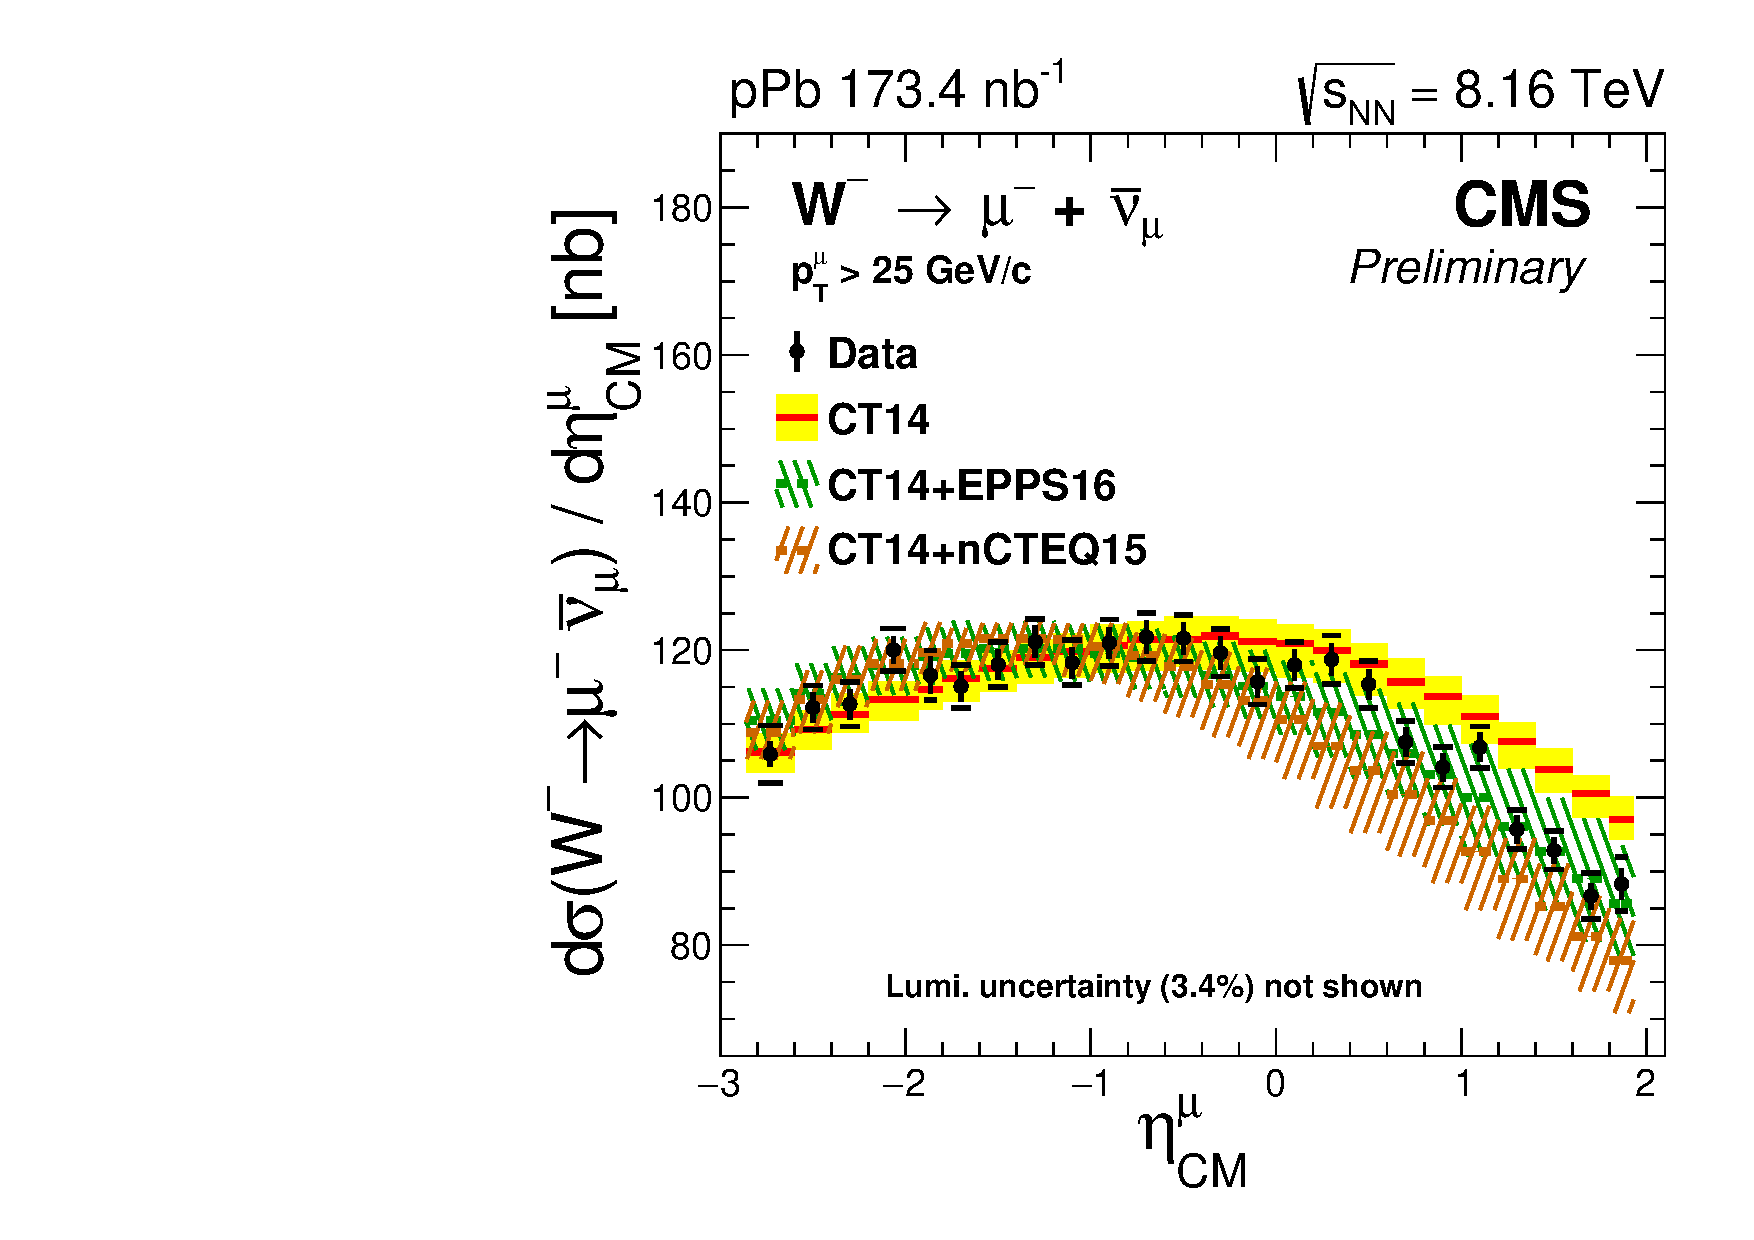
\includegraphics[width=0.45\textwidth]{Figures/WBoson/Results/Theory/Cross_Section/gr_WToMuMi_PA_Cross_Section_EffTnP_NominalWithTheory_EPPS16.pdf}
%%
  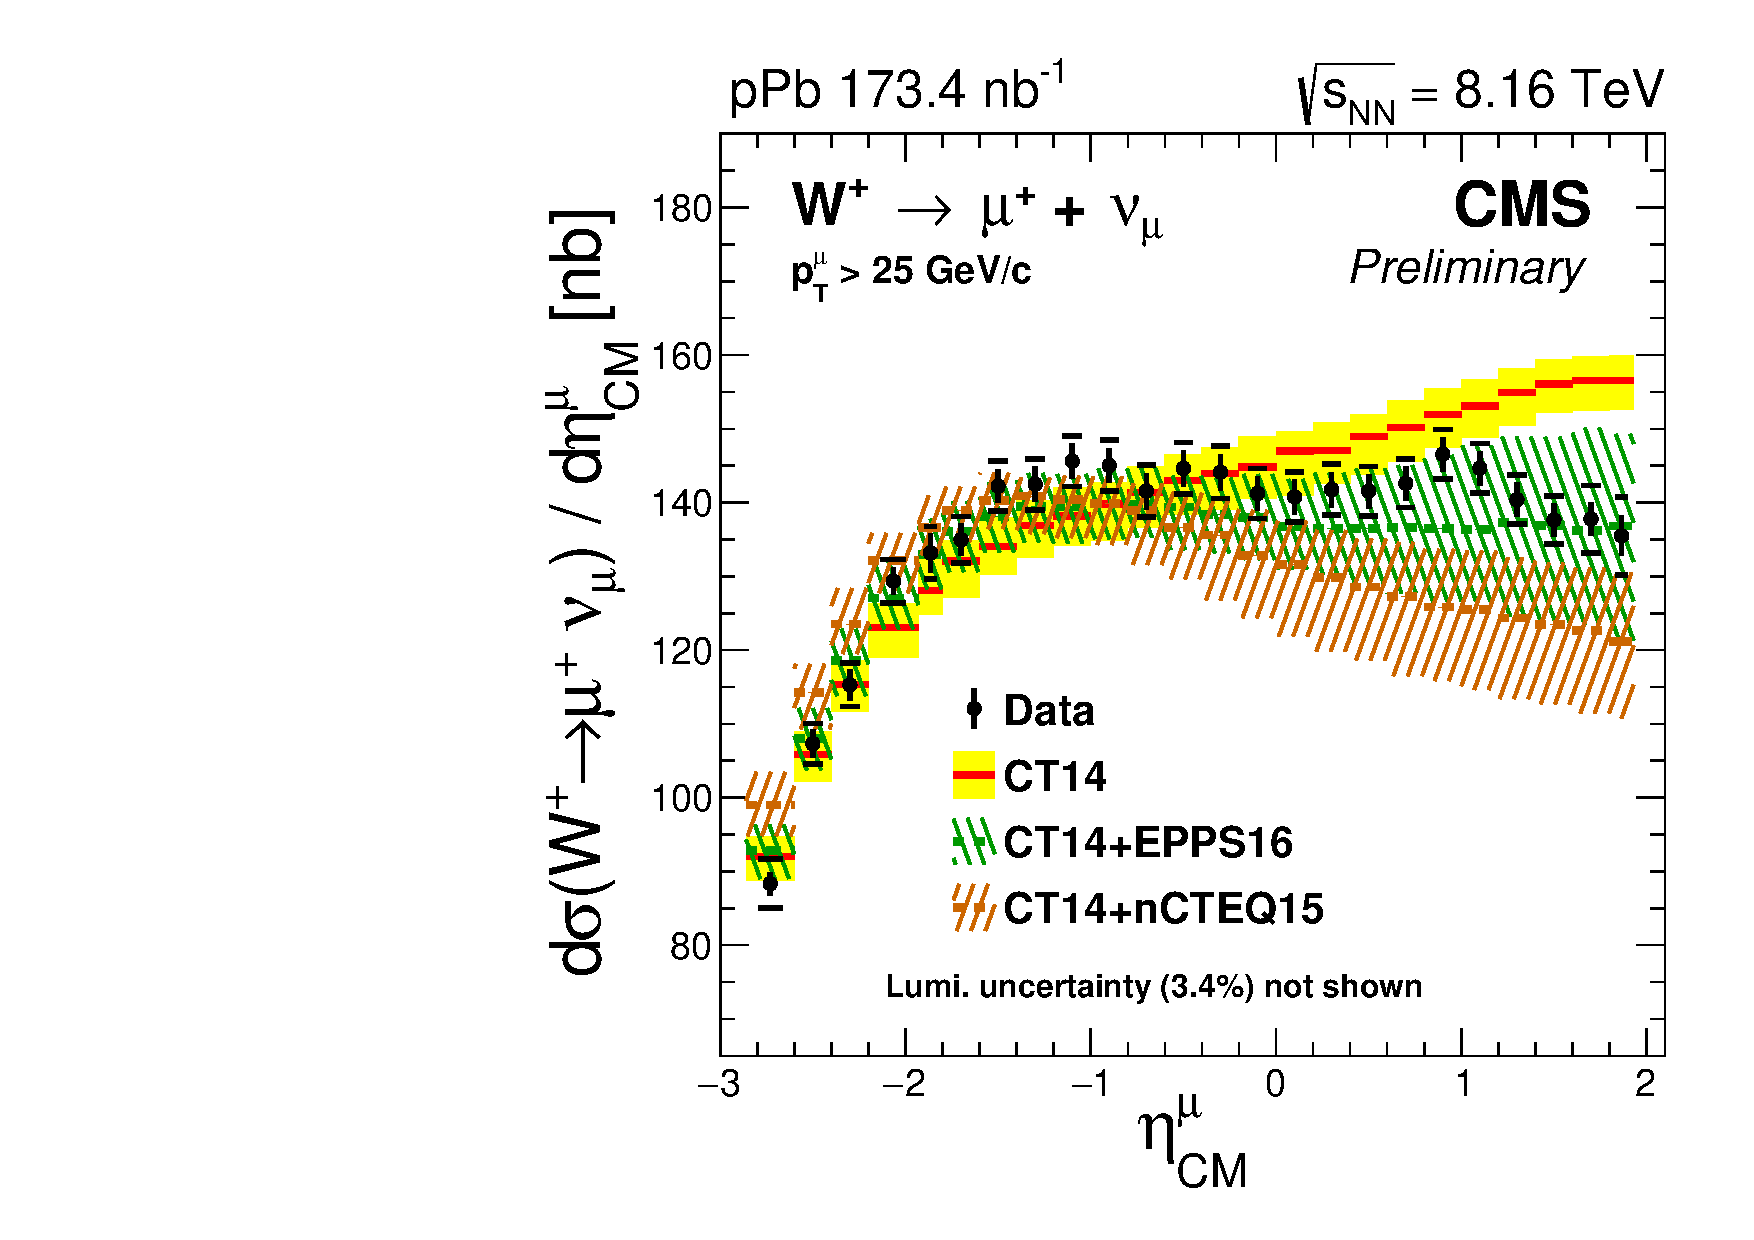
\includegraphics[width=0.45\textwidth]{Figures/WBoson/Results/Theory/Cross_Section/gr_WToMuPl_PA_Cross_Section_EffTnP_NominalWithTheory_EPPS16.pdf}
 \end{center}
 \caption{Differential cross sections for \WToMuNuPl (left) and \WToMuNuMi (right), as a function of the muon pseudorapidity in the center-of-mass frame. Errors bars represent the statistical uncertainties, while the brackets represent the statistical and systematic uncertainties summed in quadrature. The global luminosity uncertainty of $\pm$3.4\% is not displayed. Theoretical predictions with (CT14+EPPS16 shown in dashed green line and CT14+nCTEQ15 shown in dashed brown line) and without (CT14, solid red line) PDF nuclear modifications are also shown, with the uncertainty bands. All theory uncertainty bands include PDF uncertainties. }
 \label{fig:CrossSection_WToMu_PA_Model}
\end{figure}

\begin{figure}[htbp]
 \begin{center}
  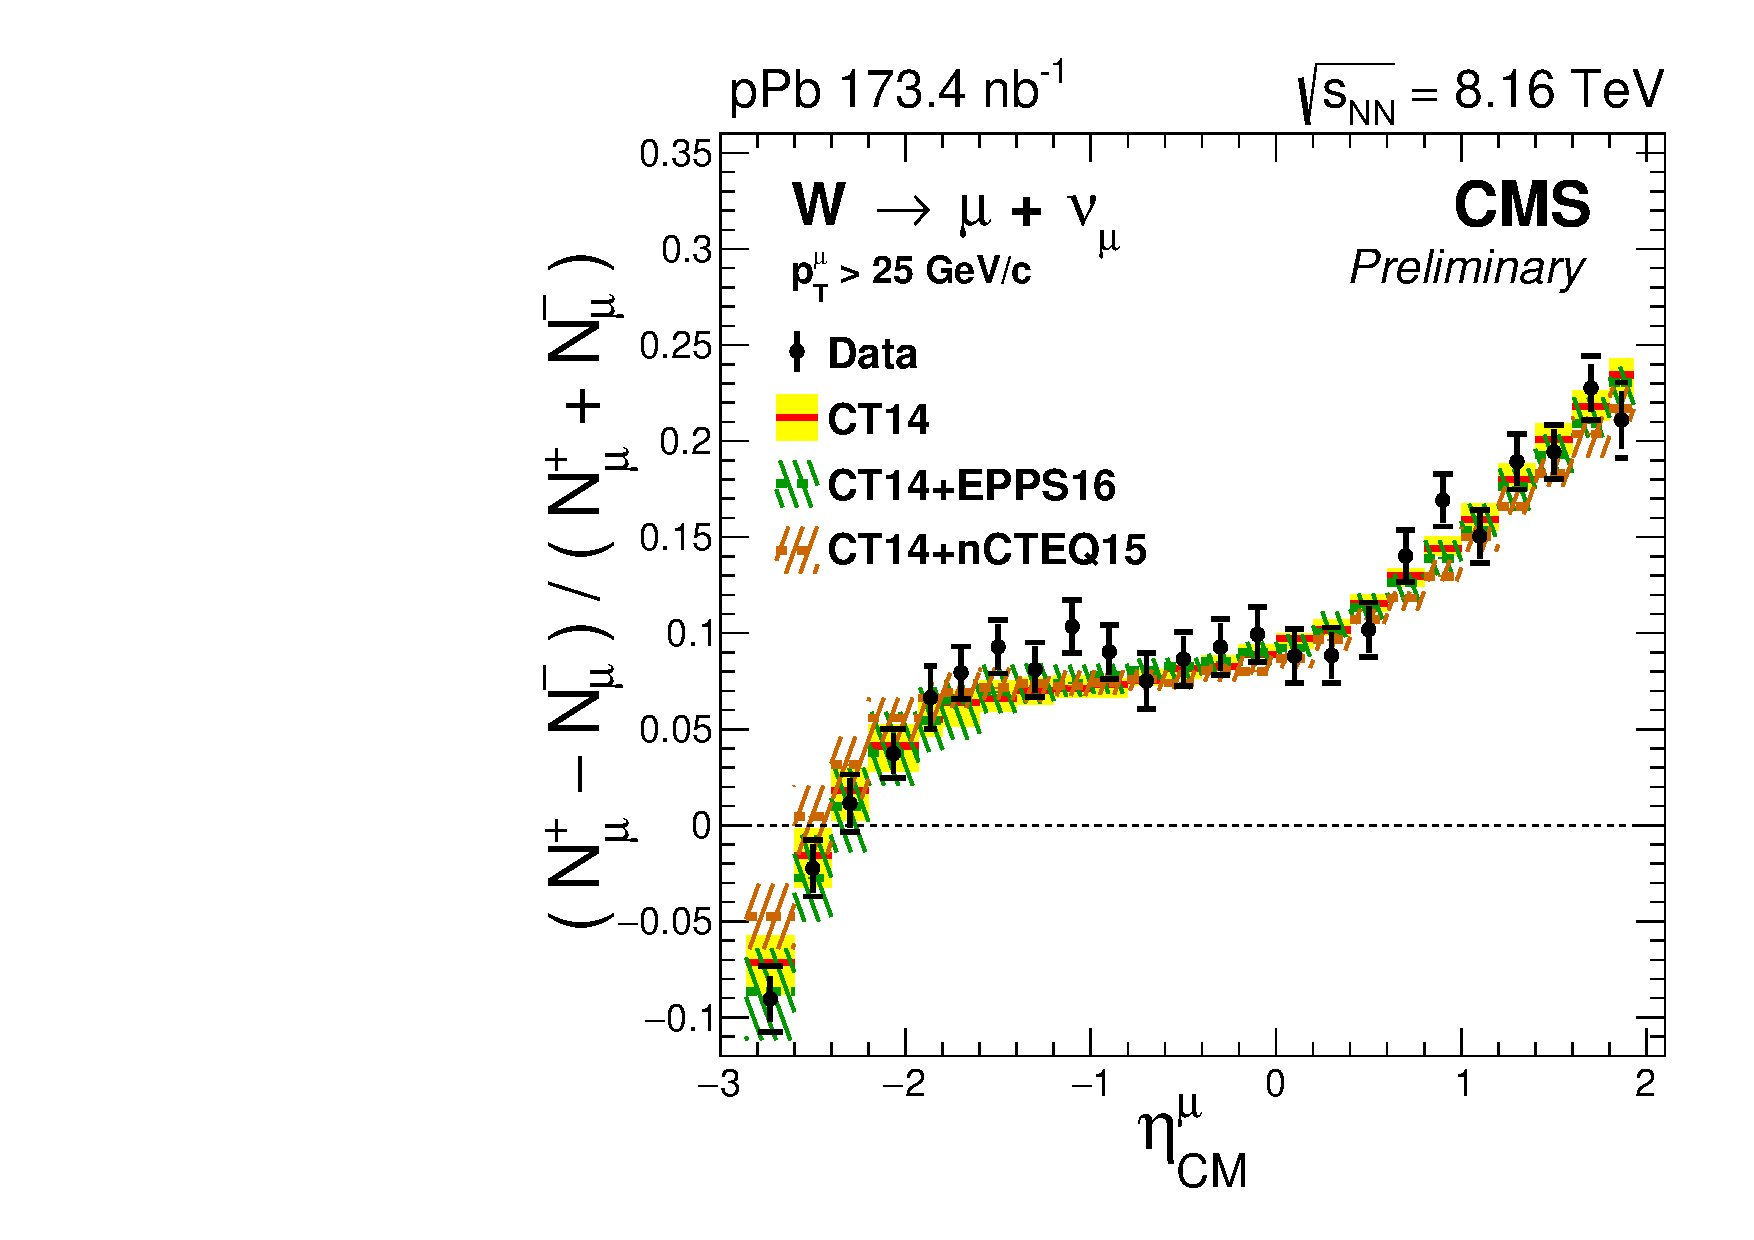
\includegraphics[width=0.45\textwidth]{Figures/WBoson/Results/Theory/Charge_Asymmetry/gr_WToMuInc_PA_Charge_Asymmetry_EffTnP_NominalWithTheory_EPPS16.pdf}
 \end{center}
 \caption{Muon charge asymmetry of $\WToMuNu$, given for each muon $\eta_{CM}$ bin. Errors bars represent the statistical uncertainties, while the brackets represent the statistical and systematic uncertainties summed in quadrature. Theoretical predictions with (CT14+EPPS16 shown in dashed green line and CT14+nCTEQ15 shown in dashed brown line) and without (CT14, solid red line) PDF nuclear modifications are also shown, with the uncertainty bands. All theory uncertainty bands include PDF uncertainties. }
 \label{fig:ChargeAsymmetry_WToMu_PA_Model}
\end{figure}


\begin{figure}[htbp]
 \begin{center}
  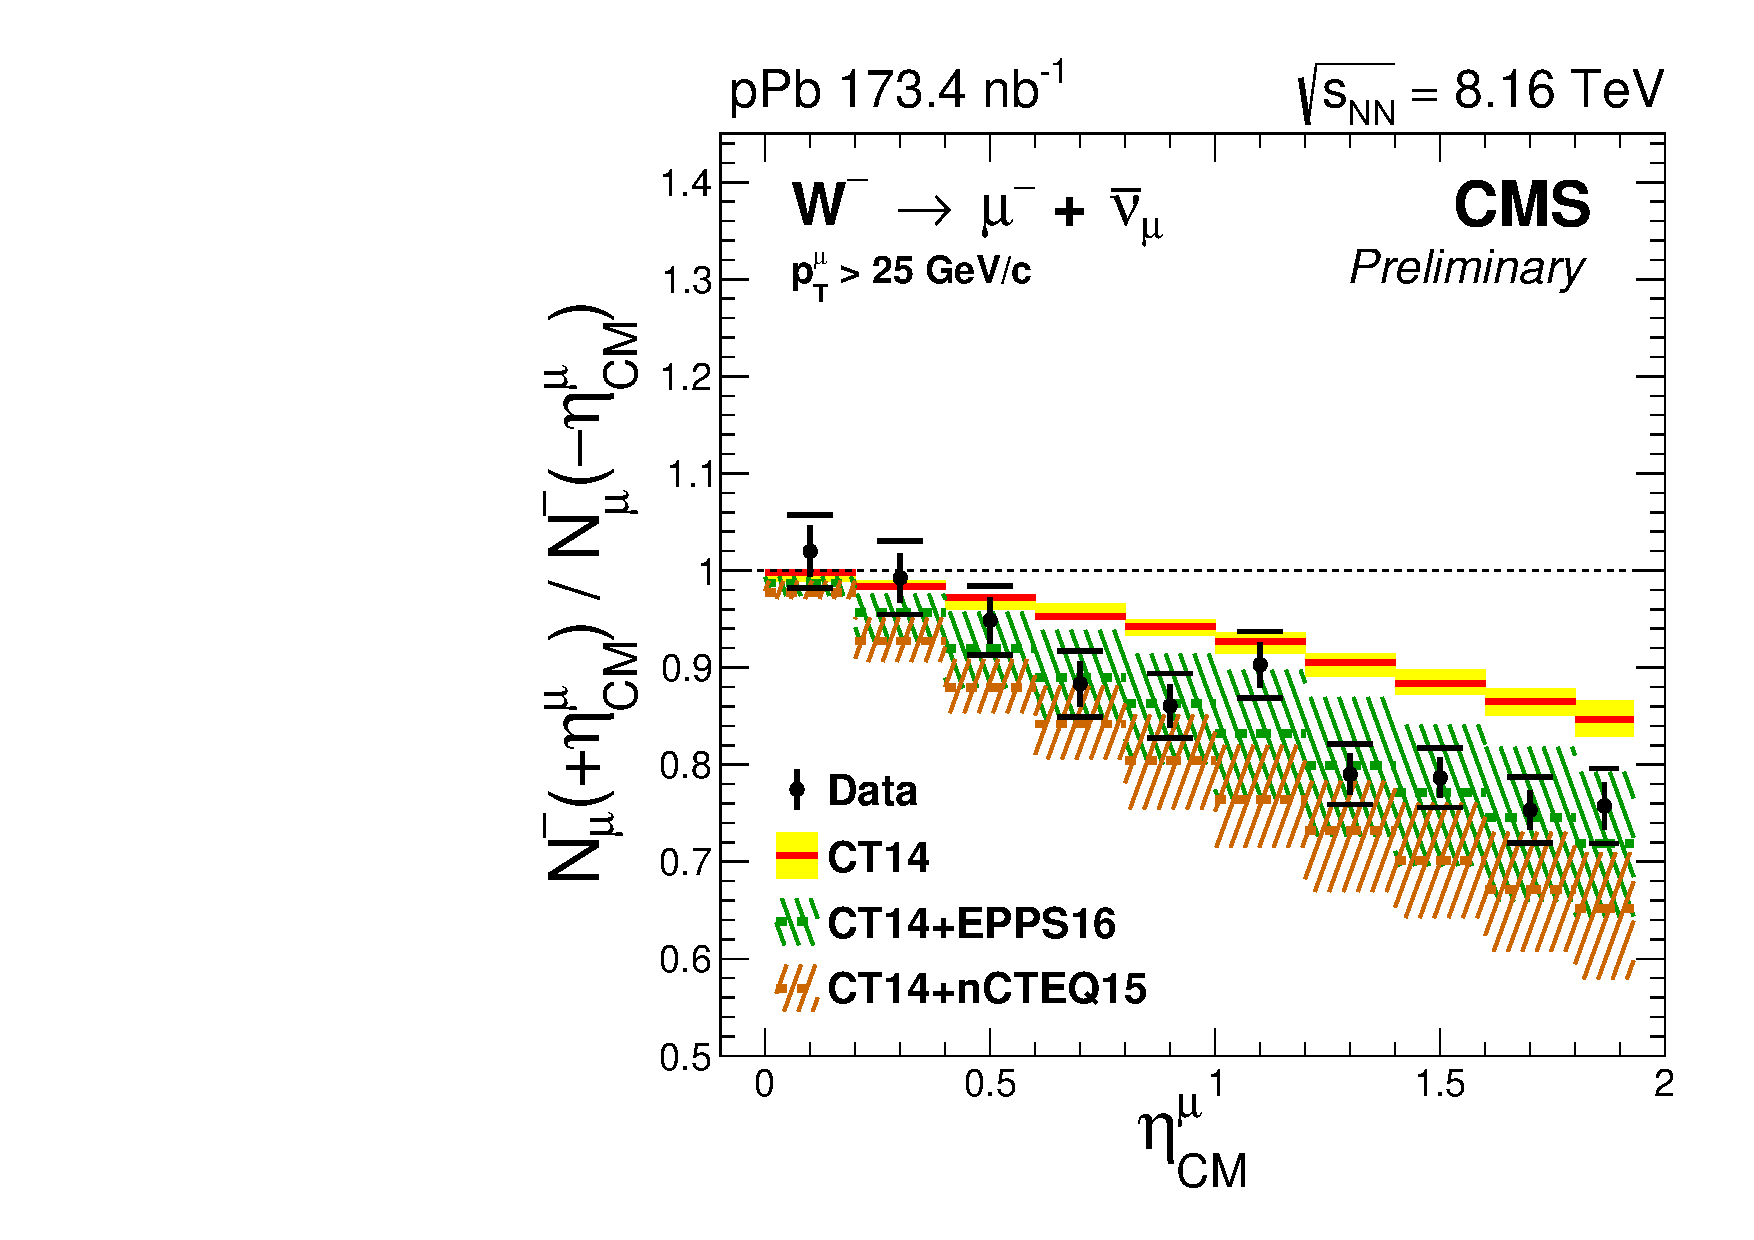
\includegraphics[width=0.32\textwidth]{Figures/WBoson/Results/Theory/ForwardBackward_Ratio/gr_WToMuMi_PA_ForwardBackward_Ratio_EffTnP_NominalWithTheory_EPPS16.pdf}
%%
  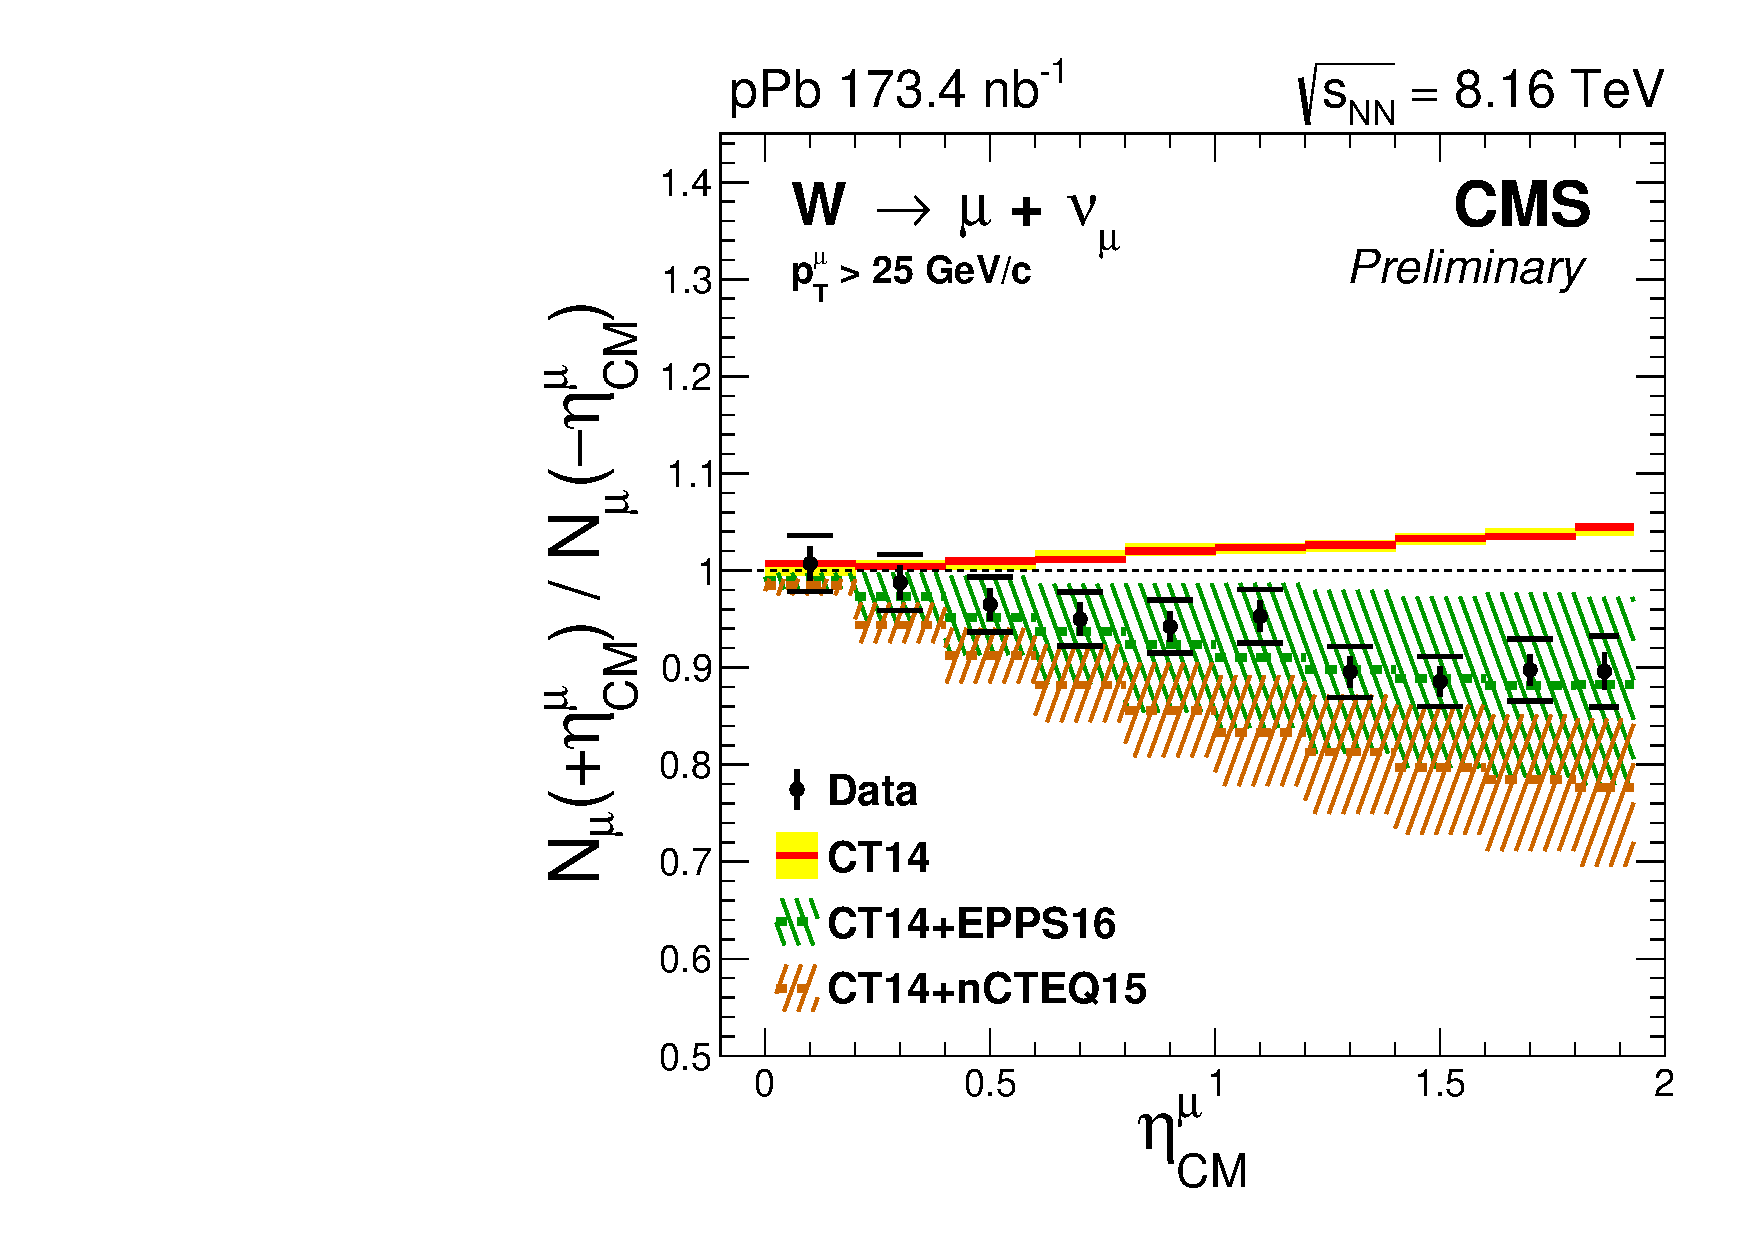
\includegraphics[width=0.32\textwidth]{Figures/WBoson/Results/Theory/ForwardBackward_Ratio/gr_WToMuInc_PA_ForwardBackward_Ratio_EffTnP_NominalWithTheory_EPPS16.pdf}
%%
  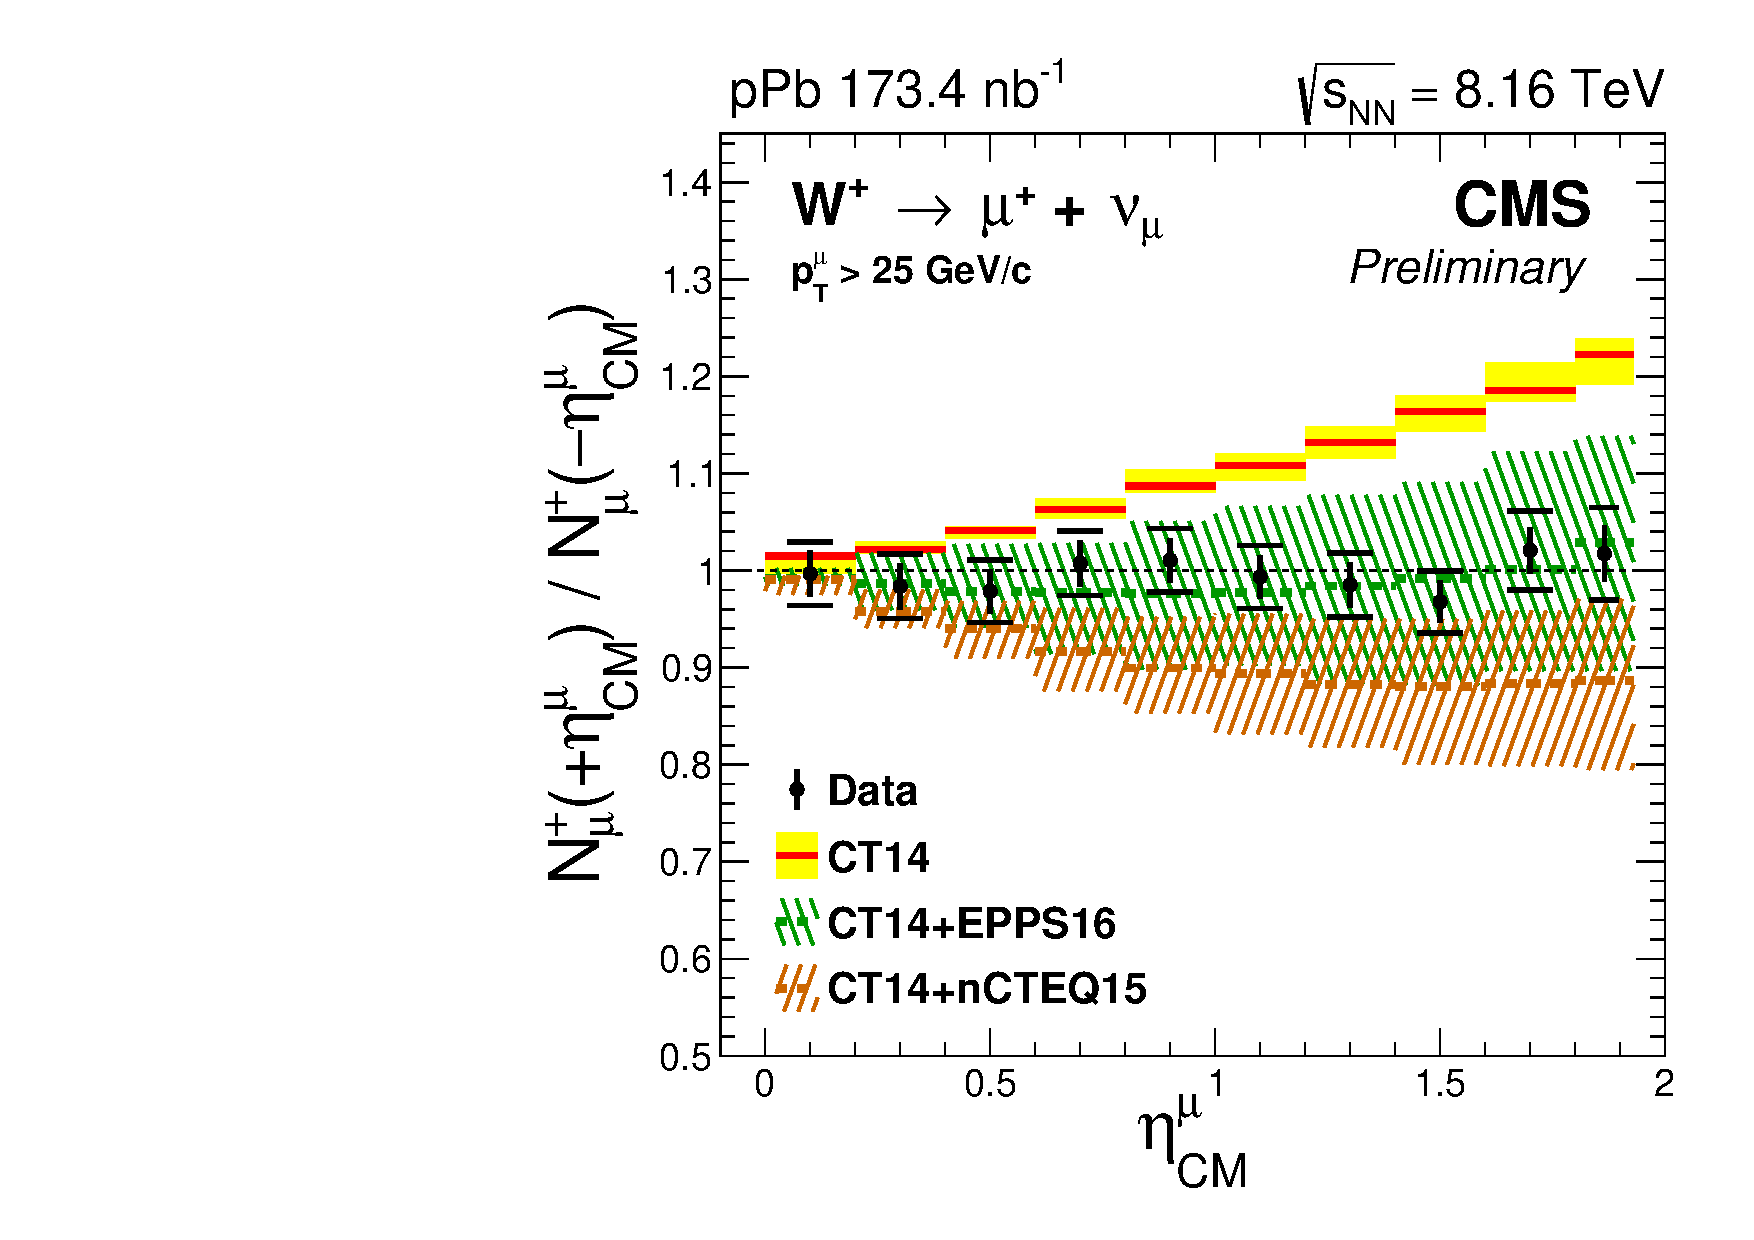
\includegraphics[width=0.32\textwidth]{Figures/WBoson/Results/Theory/ForwardBackward_Ratio/gr_WToMuPl_PA_ForwardBackward_Ratio_EffTnP_NominalWithTheory_EPPS16.pdf}
 \end{center}
 \caption{Forward-backward ratio of $\WToMuNu$, given for each muon $\eta_{CM}$ bin separated in negative (left), all (middle) and positive (right) charged muons. Errors bars represent the statistical uncertainties, while the brackets represent the statistical and systematic uncertainties summed in quadrature. Theoretical predictions with (CT14+EPPS16 shown in dashed green line and CT14+nCTEQ15 shown in dashed brown line) and without (CT14, solid red line) PDF nuclear modifications are also shown, with the uncertainty bands. All theory uncertainty bands include PDF uncertainties. }
 \label{fig:ForwardBackwardRatio_WToMu_PA_Model}
\end{figure}


In order to quantify the level of agreement between each PDF calculation and the measurements of the \W boson production in \pPb, a $\chi^{2}$ test is performed. The $\chi^{2}$ test is derived as described below:

\begin{equation}
\chi^{2} = \sum_{i}\sum_{j}\left[\left(t(i) - d(i)\right)\left(cov_{data} + cov_{theory}\right)^{-1}[i , j]\left(t(j) - d(j)\right)\right]
\label{eq:Chi2Test}
\end{equation}

where $t(i)$ is the value of the observable predicted from the PDF calculation in bin i, $d(i)$ is the value of the observable measured in data in bin i, and $\left(cov_{data} + cov_{theory}\right)^{-1}$ is the inverse of the sum of the covariance matrices extracted from the data and the model. This approach takes into account the bin-to-bin correlations in both muon charge and pseudorapidity. The outcome of the $\chi^{2}$ statistical test derived using the CT14 PDF, the CT14+EPPS16 nPDF and the CT14+nCTEQ15 nPDF calculations are summarized in \tab{tab:modelComparison_CT14}.

\begin{table}[htb!]
  \centering
  \resizebox{\textwidth}{!}{
  \renewcommand{\arraystretch}{1.5}
  \begin{tabular}{c *3c | *3c | *3c}
    \hline
    \multirow{2}{*}{Observable}  & \multicolumn{3}{c}{CT14} & \multicolumn{3}{c}{CT14+EPPS16} & \multicolumn{3}{c}{CT14+nCTEQ15} \\ \cline{2-10}
     & $\chi^{2}$ & ndf & Prob.($\%$) & $\chi^{2}$ & ndf & Prob.($\%$) & $\chi^{2}$ & ndf & Prob.($\%$) \\
    \hline
    $\dd\sigma(\WToMuNupm) / \dd\etaMuCM$ & 135 & 48 & $3\times10^{-8}$ & 32 & 48 & 96 & 40 & 48 & 79 \\
    $\left( N_{\mu}^{+} - N_{\mu}^{-} \right) \big/ \left( N_{\mu}^{+} + N_{\mu}^{-} \right)$ & 23 & 24 & 54 & 18 & 24 & 80 & 29 & 24 & 23  \\
    $N_{\mu}^{\pm}\left( +\etaMuCM \right) \big/ N_{\mu}^{\pm}\left( -\etaMuCM \right)$ & 98 & 20 & $3\times10^{-10}$ & 11 & 20 & 95 & 14 & 20 & 83  \\
    $N_{\mu}\left( +\etaMuCM \right) \big/ N_{\mu}\left( -\etaMuCM \right)$ & 87 & 10 & $2\times10^{-12}$ & 3 & 10 & 99 & 5 & 10 & 90  \\
    \hline
  \end{tabular}
  }
  \caption{Results of the $\chi^{2}$ statistical test between the measurements and the theory calculations from the CT14 PDF, CT14+EPPS16 nPDF and CT14+nCTEQ15 nPDF models. The value of the $\chi^{2}$, the number of degrees of freedom (ndf) and the $\chi^{2}$ probability (Prob.), are presented for the \WToMuNupm differential cross sections, the muon charge asymmetry, the \WToMuNupm forward-backward ratios, and the charge-summed forward-backward ratio, respectively.}
  \label{tab:modelComparison_CT14}
\end{table}





% END OF SUBSECTION




